\documentclass[conference]{IEEEtran}
\IEEEoverridecommandlockouts
% The preceding line is only needed to identify funding in the first footnote. If that is unneeded, please comment it out.
\usepackage{cite}
\usepackage{amsmath,amssymb,amsfonts}
\usepackage{algorithm}
\usepackage{algorithmic}
\usepackage{graphicx}
\usepackage{textcomp}
\usepackage{xcolor}
\usepackage{hyperref}
\hypersetup{
    colorlinks=true,
    citecolor=black,
    linkcolor=black,
    filecolor=black,      
    urlcolor=black,
    pdftitle={Online outlier Detection Threshold},
    pdfauthor={Marek Wadinger}
    pdfpagemode=FullScreen,
    }
\def\BibTeX{{\rm B\kern-.05em{\sc i\kern-.025em b}\kern-.08em
    T\kern-.1667em\lower.7ex\hbox{E}\kern-.125emX}}
\begin{document}

\title{Real-Time Outlier Detection with Dynamic Process Limits\\
% dynamic process limits

\thanks{The Authors gratefully acknowledge the contribution of the Slovak Research and Development Agency under the project APVV-20-0261. The authors gratefully acknowledge the contribution of the Scientific Grant Agency of the Slovak Republic under the grant 1/0490/23.}
}

\author{\IEEEauthorblockN{1\textsuperscript{st} Marek Wadinger}
\IEEEauthorblockA{\textit{Institute of Information Engineering, Automation and}\\ \textit{Mathematics} \\
\textit{Slovak University of Technology in Bratislava}\\
Bratislava, Slovakia \\
marek.wadinger@stuba.sk}
\and
\IEEEauthorblockN{2\textsuperscript{nd} Michal Kvasnica}
\IEEEauthorblockA{\textit{Institute of Information Engineering, Automation and}\\ \textit{Mathematics} \\
\textit{Slovak University of Technology in Bratislava}\\
Bratislava, Slovakia \\
michal.kvasnica@stuba.sk}
}

\maketitle

\begin{abstract}
In this paper, we introduce an Adaptable and Interpretable Framework for Anomaly Detection (AID) designed for industrial systems utilizing IoT data streams on top of well-established SCADA systems. AID leverages dynamic conditional probability distribution modeling to capture the normal operation of dynamic systems and isolate the root causes of anomalies at the level of individual inputs. The self-supervised framework dynamically updates parameters of underlying model, allowing it to adapt to non-stationarity. AID interprets anomalies as significant deviations from conditional probability, encompassing interactions as well as both spatial and temporal irregularities by exposing them as features. Crucially, AID provides dynamic operating limits to integrate with existing alarm handling mechanisms in SCADA-based IoT systems. Two industrial-scale case studies demonstrate AID's capabilities. The first study showcases AID's effectiveness on energy storage system, adapting to changes, setting context-aware limits for SCADA, and ability to leverage a physics-based model. The second study monitors battery module temperatures, where AID identifies hardware faults, emphasizing its relevance to energy storage safety. A benchmark evaluation on real data shows that AID delivers comparable performance to other self-learning adaptable anomaly detection methods, with the significant advancement in diagnostic capabilities for improved system reliability and performance.

\end{abstract}

\begin{IEEEkeywords}
anomaly detection, interpretable machine learning, online machine learning, real-time systems, streaming analytics
\end{IEEEkeywords}

\section{Introduction}\label{Introduction}
Anomaly detection systems play a critical role in risk-averse systems by identifying abnormal patterns and adapting to novel expected patterns in data. These systems are particularly vital in the context of Internet of Things (IoT) devices that continuously stream high-fidelity data to control units.

In this rapidly evolving field with long-spanning roots, Chandola et al. conducted an influential review of prior research efforts across diverse application domains (\cite{Chandola2009}).
Recent studies have underscored the need for holistic and tunable anomaly detection methods accessible to operators (\cite{Laptev2015, Kejariwal2015, Cook2020}).

Cook et al. denote substantial aspects that pose challenges to anomaly detection in IoT, including the temporal, spatial, and external context of measurements, multivariate characteristics, noise, and nonstationarity (\cite{Cook2020}). To address these complexity issues, Zhang et al. have successfully employed spatially distributed sensors and time-relative modulation. Their approach has proven effective, particularly in the context of complex non-linear systems, offering potential solutions to some of the challenges posed by IoT data (\cite{ZHANG2024121506}). Huang et al., on the other hand, tackled the problems of detecting global outliers, local outliers, and outlier clusters simultaneously. Their proposed approach, based on density estimation, relies on the notion that density distributions should exhibit minimal variations in local areas. To achieve this, they introduce a novel turning ratio metric, which reduces reliance on hyperparameters and enhances anomaly detection (\cite{HUANG2023120799}).

Additionally, feature engineering techniques play a crucial role in capturing contextual properties and enhancing anomaly detection performance (\cite{Fan2019}). However, it is worth noting that feature engineering may introduce categorical variables and significantly increase the dimensionality of the data, requiring specific methods for handling large data, sizeable data storage, and substantial computational resources (\cite{Talagala2021}). Recently, Li et al. introduced an attribute-weighted outlier detection algorithm, designed for high-dimensional datasets with mixtures of categorical and numerical data. Their approach assigns different weights to individual attributes based on their importance in anomaly detection and uses these weights to calculate distances between data points. Notably, Li et al. demonstrated the superior performance of their algorithm compared to state-of-the-art methods (\cite{LI2024121304}). Another strategy for handling high-dimensional data involves using deep learning methods with synthetic normal data to enhance the detection of outliers with subtle deviations, as proposed in \cite{DU2024121161}.

Nevertheless, the presence of nonstationarity, often stemming from concept drift (a shift in data patterns due to changes in statistical distribution) and change points (permanent alterations in system state), presents a substantial challenge (\cite{Salehi2018}). In practical scenarios, those changes tend to be unpredictable in both their spatial and temporal aspects. Consequently, they require systems with solid outlier rejection capabilities of intelligent tracking algorithms (\cite{Barbosa2019162}). This underscores the critical importance of an anomaly detection method's ability to adapt to evolving data structures, especially in long-term deployments. Nevertheless, as (\cite{Tartakovsky2013}) remarked, immediate detection is not a feasible option unless there is a high tolerance for false alarms.

The adaptation of batch models at scale introduces a significant latency in detector adaptation (\cite{Wu2021}). Incremental learning methods allowed adaptation while restraining the storage of the whole dataset. The supervised operator-in-the-loop solution offered by Pannu et al. showed the detector's adaptation to data labeled on the flight (\cite{Pannu2012}).
Others approached the problem as sequential processing of bounded data buffers in univariate signals (\cite{Ahmad2017134}) and multivariate systems (\cite{Bosman201514}).

\subsection{Related Work}
Recent advances in anomaly detection have broadened its scope to include root cause identification governed by the development of explanatory methods capable of diagnosing and tracking faults across the system. Studies can be split into two groups of distinct approaches. The first group approaches explainability as the importance of individual features (\cite{Carletti2019, Nguyen2019, Amarasinghe2018}). Those studies allow an explanation of novelty by considering features independently. The second group uses statistical learning creating models explainable via probability. For instance, the integration of variational Bayesian inference probabilistic graph neural network allowed Zhang et al. to model the posterior distribution of sensor dependency for gas leakage localization on unlabeled data (\cite{ZHANG2023120542}). Yang et al. recently proposed a Bayesian network (BN) for fault detection and diagnosis. In this BN, individual nodes of the network represent normally distributed variables, whereas the multiple regression model defines weights and relationships. Using the predefined structure of the BN, the authors propose offline training with online detection and diagnosis (\cite{Yang2022}).

Given the infrequent occurrence of anomalies and their potential absence in training data, the incorporation of synthetic data or feature extraction for various detected events emerges to assist diagnosis of the system. Brito et al. designed synthetic faults based on expert knowledge and introduced them into a transfer learning classifier to exploit faults in rotating machinery, with a subsequent explanation layer (\cite{BRITO2023120860}). Conversely, We et al. leveraged feature selection to expose various types of abnormal behavior. The team presents competitive performance while using change in relationships to provide causal inference (\cite{WU2024121539}).

However, it is crucial to underscore that offline training, as previously emphasized, is inherently inadequate when it comes to adapting to anticipated novel patterns, rendering it unsuitable for sustained, long-term operation on IoT devices.

This paper emphasizes the importance of combining adaptability in interpretable anomaly detection and proposes a method that addresses this challenge in real industrial systems. Here we report the discovery and characterization of an adaptive anomaly detection method for existing SCADA systems, employing streaming IoT data. The ability to diagnose multivariate data while providing root cause isolation via statistical learning, extends our previous contribution to the field as presented in (\cite{Wadinger2023}). The proposed algorithm represents a general method that aids a range of existing safety-critical systems where anomaly diagnosis and identification are paramount.

\subsection{Novelty of proposed approach}
The idea of using statistical outlier detection is well-established. We highlight the impactful contributions of Yamanishi et al. in (\cite{Yamanishi2002, Yamanishi2004}). The authors propose a method for detecting anomalies in a time series. The method is based on the assumption that the continuous data is generated by a mixture of Gaussian distributions, while discrete data is modeled as histogram density. The authors solve the problem of change point detection as well. However, the adaptation system is unaware of such changes, making the moving window the only source of adaptation. Our self-supervised approach facilitates intelligent adaptation concerning detected change points, to increase the speed of adaptation where the probability of concept drift is high. By leveraging its ability to adapt to changes in operational states, our proposed method operates autonomously when such changes occur. Moreover, \cite{Yamanishi2004} does not attempt to isolate the root cause of the anomaly. Our approach extends statistical outlier detection by incorporating interpretability. This is achieved by evaluating the inverse cumulative distribution function of the latest conditional probabilities for each measurement, considering the remainder of the measurements, and establishing limits that define the threshold for normal event probabilities.

A limited number of studies have focused on adaptation and interpretability within the framework of anomaly detection. Two recent contributions in this area are made by Steenwinckel et al. as reported in (\cite{Steenwinckel2018, Steenwinckel2021}). In \cite{Steenwinckel2018}, the authors emphasize the importance of combining prior knowledge with a data-driven approach to achieve interpretability, particularly concerning root cause isolation. They propose a novel approach that involves extracting features based on knowledge graph pattern extraction and integrating them into the anomaly detection mechanism. This graph is subsequently transformed into a matrix, and adaptive region-of-interest extraction is performed using reinforcement learning techniques. To enhance interpretability, a Generative Adversarial Network (GAN) reconstructs a new graphical representation based on selected vectors. However, it is important to note that the validation of this idealized approach is pending further investigation. Lately, \cite{Steenwinckel2021} introduced a comprehensive framework for adaptive anomaly detection and root cause analysis in data streams. While the adaptation process is driven by user feedback, the specific mechanism remains undisclosed. The authors present an interpretation of their method through a user dashboard, featuring visualizations of raw data. This dashboard is capable of distinguishing between track-related problems and train-related issues, based on whether multiple trains at the same geographical location approach the anomaly. Meanwhile, our efforts are directed towards the development of a self-supervised method that can learn autonomously, reducing the reliance on human supervision, which is often constrained by time limitations and can lead to significant delays in adaptation. Our method is distinguished by its straightforward statistical reasoning and the ability to isolate the root cause of anomalies. The interpretability of our method is demonstrated through the establishment of dynamic process limits for each signal, leveraging conditional probabilities derived from the signal and other system measurements and features. This provides operators with a clear understanding of the system's state and the underlying causes of anomalies and aids existing alarm handling mechanisms in SCADA which utilize process limits. To the best of our knowledge, this is the first study to propose a self-supervised method for adaptive anomaly detection and root cause isolation in streaming IoT data.

\subsection{Broader Impact}
Potential applications of the proposed method are in the field of energy storage systems, where the ability to detect anomalies and isolate their root causes while adapting to changes in operation and environment, is crucial for the system safety. The proposed method is designed to be integrated into the existing infrastructure of the systems, utilizing IoT data streams on top of well-established SCADA systems. SCADA systems continuously monitor these process data in real-time, embodying alarm handling mechanisms, which are designed to notify operators of the system's abnormal behavior and drive attention to the root of the problem. By comparing the current values to the upper and lower process limits, they take action when a variable exceeds or falls below these limits. However, safe operating limits are often established based on a combination of equipment design limits and the dynamics of the process (\cite{Stauffer2021}). Those are indifferent to the actual state of the system and environmental conditions. The proposed method allows the establishment of dynamic process limits, which are based on the current state of the system and its environment. This allows the system to operate closer or further from its design limits, increasing its safety and profitability. The dynamic process limits allow operational metrics monitoring, making potential early detection and prevention easier. Using adaptable methods without interpretability, on the other hand, may pose safety risks and lower total financial benefits, as the triggered false alarms may need to be thoroughly analyzed, resulting in prolonged downtimes.

\subsection{Validation}\label{par:validation}
Two case studies show that our proposed method has the capacity to explain anomalies, isolate the root cause, and allow adaptation to change points, advancing recently developed anomaly detection techniques for long-term deployment and cross-domain usage. We observe similar detection performance, albeit with lower scalability, on benchmark data when comparing our approach to well-established unsupervised anomaly detection methods in streamed data which create a bedrock for many state-of-the-art contributions, such as One-Class SVM (\cite{Amer2013, Liu2014, Krawczyk2015, Miao2019, Gozuacik2021}), and Half-Space Trees (\cite{Wetzig2019, Lyu2020}).


The main contribution of the proposed solution to the developed body of research is that it:
\begin{itemize}
\item Enriches interpretable anomaly detection with adaptive capabilities
\item Isolates root cause of anomalies while considering interactions
\item Uses self-learning approach on streamed IoT data
\item Demonstrates interpretability by providing process limits for signals
\item Blends with existing SCADA architecture
\end{itemize}

\subsection{Paper Organization}
The rest of the paper is structured as follows: We begin with the problem and motivation in \textbf{Section~\ref{Introduction}}, providing context. Next, in \textbf{Section~\ref{Preliminaries}}, we lay the theoretical groundwork. Our proposed adaptive anomaly detection method is detailed in \textbf{Section~\ref{Proposed Method}}. We then demonstrate real-world industrial-scale applications in \textbf{Section~\ref{Case Study}}. Finally, we conclude the paper in \textbf{Section~\ref{Conclusion}}, summarizing findings and discussing future research directions.



\section{Preliminaries}
In this section, we present the fundamental ideas that form the basis of the developed approach. Subsection \ref{AA:Welford} explains Welford's online algorithm, which can adjust distribution to changes in real-time. Subsection \ref{AA:InvWelford} proposes a two-pass implementation that can reverse the impact of expired samples. The math behind distribution modeling in Subsection \ref{AA:Distribution} establishes the foundation for the Gaussian anomaly detection model discussed in Subsection \ref{AA:Anomaly}, followed by conditional probability computation in Subsection \ref{AA:Conditional}. The last subsection of the preliminaries is devoted to the definition of anomalies.

\subsection{Welford's Online Algorithm}\label{AA:Welford}
Welford introduced a numerically stable online algorithm for calculating mean and variance in a single pass through data. Therefore, the algorithm allows the processing of IoT device measurements without the need to store their values \cite{Wel62}.

Given measurement \(x_i\) where \(i=1,...,n\) is a sample index in sample population \(n\), the corrected sum of squares \(S_n\) is defined as
\begin{equation}
S_n = \sum_{i=1}^n (x_i - \bar x_n)^2\text{,}\label{eq:sumsquares}
\end{equation}
with the running mean \(\bar x_n\) defined as previous mean \(\bar x_{n-1}\) weighted by proportion of previously seen population \(n-1\) corrected by current sample as
\begin{equation}
\bar x_n = \frac{n-1}{n} \bar x_{n-1} + \frac{1}{n}x_n = \bar x_{n-1} + \frac{x_n - \bar x_{n-1}}{n}\text{.}\label{eq:runmean}
\end{equation}
Throughout this paper, we consider the following formulation of an update to the corrected sum of squares:
\begin{equation}
S_n = S_{n-1} + (x_n - \bar x_{n-1})(x_n - \bar x_n)\text{,}\label{eq:upsumsquares}
\end{equation}
as it is less prone to numerical instability due to catastrophic cancellation, significant loss of precision due to subtracting two nearly equal numbers. Finally, the corresponding unbiased variance is
\begin{equation}
s^2_n = \frac{S_{n}}{n-1}\text{.}\label{eq:runvar}
\end{equation}

This implementation of the Welford method requires the storage of three scalars: \(\bar x_{n-1}\); \(n\); \(S_n\).

\subsection{Inverting Welford's Algorithm}\label{AA:InvWelford}
Based on \eqref{eq:runmean}, it is clear that the influence of the latest sample over the running mean decreases as the population \(n\) grows. For this reason, regulating the number of samples used for sample mean and variance computation has crucial importance over adaptation. Given access to the instances used for computation and expiration period \(\ui{t}{e} \in \mathbb{N}_{0}^{n-1}\), reverting the impact of \(x_{n-\ui{t}{e}}\) can be written as follows

\begin{equation}
S_{n-1} = S_n - (x_{n-\ui{t}{e}} - \bar x_{n-1})(x_{n-\ui{t}{e}} - \bar x_n)\text{,}\label{eq:revrunmean}
\end{equation}

where the reverted mean is given as

\begin{equation}
\bar x_{n-1} = \frac{n}{n-1} \bar x_{n} - \frac{1}{n-1}x_{n-\ui{t}{e}} = \bar x_{n} - \frac{x_{n-\ui{t}{e}} - \bar x_{n}}{n-1}\text{.}\label{eq:revmean}
\end{equation}


Finally, the unbiased variance follows the formula:

\begin{equation}
s^2_{n-1} = \frac{S_{n-1}}{n-2}\text{.}\label{eq:revvar}
\end{equation}

Notably, inversion allows the algorithm to keep constant rate of adaptation at cost of storing a bounded data buffer.

\subsection{Statistical Model of Multivariate System}\label{AA:Distribution}
Multivariate normal distribution generalizes the multivariate systems to the model where the degree to which variables are related is represented by the covariance matrix. Gaussian normal distribution of variables is a reasonable assumption for process measurements, as it is a common distribution that arises from stable physical processes measured with noise (\cite{Mishra201831}). The general notation of multivariate normal distribution is:
\begin{equation}
 \mathbf{X}\ \sim\ \mathcal{N}_k(\boldsymbol\mu,\, \boldsymbol\Sigma)\text{,}\label{eq:distribution}
\end{equation}

where $k$-dimensional mean vector is denoted as \(\boldsymbol\mu = (\bar x_{1},...,\bar x_{k})^T\ \in \mathbb{R}^{k}\) and \(\boldsymbol\Sigma \in \mathbb{R}^{k\times{k}}\) is the $k \times k$ covariance matrix, where \(k\) is the index of last random variable.

The probability density function (PDF) \(f(\boldsymbol{x}; \boldsymbol{\mu}, \boldsymbol{\Sigma})\) of multivariate normal distribution is denoted as:
\begin{equation}
f(\boldsymbol{x}; \boldsymbol{\mu}, \boldsymbol{\Sigma}) = \frac{1}{(2\pi)^{k/2} |\boldsymbol{\Sigma}|^{1/2}} e^{-\frac{1}{2} (\boldsymbol{x}-\boldsymbol{\mu})^\top \boldsymbol{\Sigma}^{-1} (\boldsymbol{x}-\boldsymbol{\mu})}\text{,}
\end{equation}

where $\boldsymbol{x}$ is a $k$-dimensional vector of measurements $x_i$ at time $i$, $|\boldsymbol{\Sigma}|$ denotes the determinant of $\boldsymbol{\Sigma}$, and $\boldsymbol{\Sigma}^{-1}$ is the inverse of $\boldsymbol{\Sigma}$.

The cumulative distribution function (CDF) of a multivariate Gaussian distribution describes the probability that all components of the random vector \(\boldsymbol{X}\) take on a value less than or equal to a particular point \(q\) in space, and can be used to evaluate the likelihood of observing a particular set of measurements or data points. In other words, it gives the probability of observing a random vector that falls within a certain region of space. The standard notation of CDF is as follows:

\begin{equation}
F(\boldsymbol{x}; \boldsymbol{\mu}, \boldsymbol{\Sigma}) = \int_{-\infty}^{q} f(\boldsymbol{x}; \boldsymbol{\mu}, \boldsymbol{\Sigma}) \text{d}\boldsymbol{x}\text{,}\label{eq:cdf}
\end{equation}

where $\text{d}\boldsymbol{x}$ denotes the integration over all $k$ dimensions of $\boldsymbol{x}$.

As the equation \eqref{eq:cdf} cannot be integrated explicitly, an algorithm for numerical computation was proposed in \cite{Genz2000}.

Given the PDF, we can also determine the value of \(\boldsymbol{x}\) that corresponds to a given quantile $q$ using a numerical method for inversion of CDF (ICDF) often denoted as percent point function (PPF) or $F(\boldsymbol{x}; \boldsymbol{\mu}, \boldsymbol{\Sigma})^{-1}$. An algorithm that calculates the value of the PPF is part of standard statistical software tools.

\subsection{Conditional Probability Distribution}\label{AA:Conditional}
% https://statproofbook.github.io/P/mvn-cond.html
% @misc{https://doi.org/10.5281/zenodo.4305950,
% doi = {10.5281/ZENODO.4305950},
% url = {https://zenodo.org/record/4305950},
% author = {Soch, Joram and Proofs, The Book Of Statistical and Faulkenberry, Thomas J. and Petrykowski, Kenneth and Allefeld, Carsten},
% title = {StatProofBook/StatProofBook.github.io: StatProofBook 2020},
% publisher = {Zenodo},
% year = {2020},
% copyright = {Open Access}
% }
Considering that we observe particular vector $\boldsymbol{x}_i$, we can update probability distributions, calculated according to the rules of conditional probability, of individual measurements within the vector given the rest of the measurements in $\boldsymbol{x_{i}}$.
Let's assume multivariate normal distribution \eqref{eq:distribution} and without loss of generality, that the vector $\boldsymbol{x}_i$ can be partitioned into subset variable $x_a$, and complement vector $\boldsymbol{x_b}$ as follows

\begin{equation}
 \boldsymbol{x}_i = \begin{bmatrix}x_a \\ \boldsymbol{x_b} \end{bmatrix} \text{with dimensions} \begin{bmatrix}1\times 1 \\ (k - 1) \times 1\end{bmatrix} \text{,}
\end{equation}

where $a = 1,...,k$ and $\boldsymbol{b} = \{1, 2, \ldots, k\} \text{ where }a \notin \boldsymbol{b}$. This partitioning allows us to define block-wise mean and covariance as follows:

\begin{equation}
 \boldsymbol\mu = \begin{bmatrix}\mu_a \\ \boldsymbol{\mu_b} \end{bmatrix} \text{with dimensions} \begin{bmatrix}1\times 1 \\ (k - 1) \times 1\end{bmatrix} \text{,}
\end{equation}
and
\begin{equation}
 \boldsymbol\Sigma = \begin{bmatrix}\sigma_{aa}^2 & \boldsymbol\Sigma_{a\boldsymbol{b}} \\ \boldsymbol\Sigma_{\boldsymbol{b}a} & \boldsymbol\Sigma_{\boldsymbol{bb}} \end{bmatrix}
 \text{with dimensions} \begin{bmatrix}1\times 1 & 1\times (k - 1) \\ (k - 1) \times 1 & (k - 1) \times (k - 1)\end{bmatrix} \text{.} \label{eq:sigma}
\end{equation}

Subsequently, we can derive the conditional distribution of any subset variable $x_a$, given the complementary vector $\boldsymbol{x_b}$. This conditional distribution conforms to a univariate normal distribution, characterized by:

\begin{equation}
  X_a \mid \mathbf{X}_{\boldsymbol{b}} \sim\ \mathcal{N}(\mu_{a \mid \boldsymbol{b}},\, \sigma_{a \mid \boldsymbol{b}}^2)\text{.}\label{eq:cond_distribution}
\end{equation}

where $\mu_{a \mid \boldsymbol{b}}$ denotes the conditional mean and $\sigma_{a \mid \boldsymbol{b}}^2$ represents the conditional variance. These crucial parameters can be computed applying the Schur complement as follows:

\begin{equation}
  \sigma_{a \mid \boldsymbol{b}}^2 = \sigma_{aa}^2 - \boldsymbol\Sigma_{a\boldsymbol{b}} \boldsymbol\Sigma_{\boldsymbol{bb}}^{-1} \boldsymbol\Sigma_{\boldsymbol{b}a}\text{,}\label{eq:cond_var}
\end{equation}

for the conditional variance $\sigma_{a \mid \boldsymbol{b}}^2$, while the conditional mean, denoted as $\mu_{a \mid \boldsymbol{b}}$, is determined by:

\begin{equation}
  \mu_{a \mid \boldsymbol{b}} = \mu_a + \boldsymbol\Sigma_{a\boldsymbol{b}} \boldsymbol\Sigma_{\boldsymbol{bb}}^{-1} (\boldsymbol{x_b} - \boldsymbol\mu_b)\text{.}\label{eq:cond_mean}
\end{equation}

The conditional variance $\sigma_{a \mid \boldsymbol{b}}^2$ essentially represents the Schur complement of $\boldsymbol\Sigma_{\boldsymbol{bb}}$ within the overall covariance matrix $\boldsymbol\Sigma$.

\subsection{Gaussian Anomaly Detection}\label{AA:Anomaly}
From a viewpoint of statistics, outliers are commonly denoted as values that significantly deviate from the mean. Under the assumption that the spatial and temporal characteristics of a system, observed over a moving window, can be suitably represented as normally distributed features, we assert that any anomaly can be identified as an outlier.

In empirical fields like machine learning, the three-sigma rule ($3\sigma$) provides a framework for characterizing the region of a distribution within which normal values are expected to fall with high confidence. This rule renders approximately 0.265\% of values in the distribution as anomalous.

The \(3\sigma\) rule establishes the probability that any sample \(x_a\) of a random vector \({X}\) falls within a given CDF over a semi-closed interval as the distance from the conditional mean \(\mu_{a \mid \boldsymbol{b}} \) of 3 conditional variances \(\sigma_{a \mid \boldsymbol{b}}^2\) and gives an approximate value of $q$ as
\begin{equation}
q=P\{|x_a-\mu_{a \mid \boldsymbol{b}} |<3\sigma_{a \mid \boldsymbol{b}}^2\}=0.99735
\text{.}\label{eq:q}
\end{equation}

Utilizing a probabilistic model of normal behavior, we can determine threshold values ${\ui{x}{l}}$ and ${\ui{x}{u}}$ corresponding to the closed interval of the CDF where this probability is established. The inversion of Equation \eqref{eq:cdf} facilitates this calculation, yielding:

\begin{equation}
{\ui{x}{l}} = F((1 - P\{|x_a-\mu_{a \mid \boldsymbol{b}}|<3\sigma_{a \mid \boldsymbol{b}}^2\}); \mu_{a \mid \boldsymbol{b}}, \sigma_{a \mid \boldsymbol{b}}^2)^{-1}\text{,}\label{eq:thresh_low}
\end{equation}

for the lower limit, and

\begin{equation}
{\ui{x}{u}} = F((P\{|x_a-\mu_{a \mid \boldsymbol{b}}|<3\sigma_{a \mid \boldsymbol{b}}^2\}); \mu_{a \mid \boldsymbol{b}}, \sigma_{a \mid \boldsymbol{b}}^2)^{-1}\text{,}\label{eq:thresh_high}
\end{equation}

for the upper limit. These lower and upper limits together form vectors $\boldsymbol{\ui{x}{l}}$ and $\boldsymbol{\ui{x}{u}}$, respectively, defining the region of normal system operation. This region is conceptualized as a hypercube in the feature space, with each dimension bounded by the corresponding feature limits, as computed using Equations \eqref{eq:thresh_low} and \eqref{eq:thresh_high} for all $a = 1,...,k;~ \boldsymbol{b} = \{1, 2, \ldots, k\}$ where $a \notin \boldsymbol{b}$. The approximation of a confidence ellipse as a hypercube can be employed to represent the region of normal system operation for individual variables of a multivariate system, rendering it as an aid for visual representation.

The predicted state of the system, denoted as $y_i$, and the normality of signals $\uis{\boldsymbol{y}}{s}{i}$ at time $i$ are determined based on the maximum distance of observations from the center of the probabilistic density. The center of the probabilistic density corresponds to the vector of conditional means $\mu_{a \mid \boldsymbol{b}}$ with respect to other features. The calculation of this distance involves the cumulative distribution function (CDF) of observations and conditional distributions, as  follows:

% https://stats.stackexchange.com/questions/186402/expressing-conditional-covariance-matrix-in-terms-of-covariance-matrix

\begin{equation}
 {F(x_a; \mu_{a \mid \boldsymbol{b}}, \sigma_{a \mid \boldsymbol{b}}^2)}:a = 1,...,k;~ \boldsymbol{b} = \{1, 2, \ldots, k\} \text{ where }a \notin \boldsymbol{b} \text{.}\label{eq:max_score}
\end{equation}

Subsequently, operation states of individual inputs are defined as follows:

\begin{equation}
 \uis{\boldsymbol{y}}{s}{i} =
 \begin{cases}
 0 & \text{ if } T \leq \eqref{eq:max_score}
 \\
 1 & \text{ if } T > \eqref{eq:max_score}
 \text{,}\label{eq:anomaly_signal}
 \end{cases}
\end{equation}

where $T$ represents a threshold that distinguishes between normal signal measurement ($\uis{\boldsymbol{y}}{s}{i} = 0$) and abnormal ($\uis{\boldsymbol{y}}{s}{i} = 1$).

For the overall abnormality of the system, any anomaly in signals $\uis{\boldsymbol{y}}{s}{i}$ is considered, resulting in:

\begin{equation}
 y_i =
 \begin{cases}
 1 & \text{if } 1 \in \uis{\boldsymbol{y}}{s}{i}
 \\
 0 & \text{otherwise}
 \text{,}\label{eq:anomaly}
 \end{cases}
\end{equation}


defining the discrimination boundary between system operation where $y_i = 0$ indicates normal system operation, and $y_i = 1$ indicates anomalous operation.

\subsection{Anomaly Definition}\label{AA:AnomalyDefinition}
This subsection provides an overview of the definition of anomalies in data analysis and their categorization, setting convention for this paper.

In the realm of data analysis, anomalies are conspicuous deviations from the anticipated patterns within a dataset. Traditionally, the task of anomaly detection has relied upon unsupervised methodologies, wherein the identification of "outliers" entails the comparison of data points in both temporal and spatial contexts. This approach, often referred to as point-wise anomaly detection, classifies a data point as an anomaly when it exhibits significant dissimilarity from its neighboring data points (\cite{IGLESIASVAZQUEZ2023120994}).

The concept of point anomalies, influenced by factors such as temporal and spatial aspects, can be further categorized into conditional and contextual anomalies (\cite{Ruff2021}).

Nevertheless, this conventional method may not be suitable for scenarios characterized by collective anomalies, where clusters of abnormal data points coexist. A more pragmatic approach defines anomalies as deviations from established "normal" patterns, resembling the principles of semi-supervised learning. Change point detection, in a similar vein, can be regarded as a relative approach that takes into account the varying dynamics of changes, whether they occur gradually or abruptly (\cite{IGLESIASVAZQUEZ2023120994}).

It is imperative to recognize that the interpretation of anomalies, outliers, and novelties can vary upon the application. Anomalies typically garner significant attention, while outliers are often treated as undesirable noise and are typically excluded during data preprocessing. Novelties, on the other hand, signify new observations that necessitate model updates to adapt to an evolving environment (\cite{Ruff2021}).

Notwithstanding the differences in terminology, methods employed for the identification of data points residing in low-probability regions, irrespective of whether they are referred to as "anomaly detection," "outlier detection," or "novelty detection," share fundamental similarities (\cite{IGLESIASVAZQUEZ2023120994}).


\section{ICDF-based Real-Valued Threshold System}
In this section, we propose an adaptive and interpretable detection framework (AID) for multivariate systems with streaming IoT devices. This approach models the system as a dynamic joint normal distribution, enabling it to effectively adapt to pervasive nonstationary effects on processes. Our method handles various factors, including change points, concept drift, and seasonal effects. Our primary contribution lies in the fusion of an adaptable self-supervised system with root cause identification capabilities. This combination empowers the online statistical model to diagnose anomalies through two distinct mechanisms. Firstly, it employs conditional probability calculations to assess the system's operating conditions' normality. Secondly, it identifies outliers within individual signal measurements and features based on dynamic alert-triggering process limits. In the following sections, we describe our proposed methodology across three subsections. The initial subsection delves into the process of initializing the model's parameters. The subsequent section describes online training and adaptation, while the final subsection expounds upon the model's detection and diagnostic capabilities. For a concise representation of the proposed method, Algorithm \ref{alg:detector} is provided.

\subsection{Model Parameters Initialization}\label{init}
The model initialization is governed by defining two tunable hyperparameters of the model: the expiration period ($\ui{t}{e}$) and the threshold ($T$). The expiration period determines the window size for time-rolling computations, impacting the proportion of outliers within a given timeframe, and directly influencing the relaxation (with a longer expiration period) or tightening (with a shorter expiration period) of dynamic signal limits. Additionally, we introduce a grace period, which defaults to $3/4 \ui{t}{e}$, allowing for model calibration. During this grace period, system anomalies are not flagged to prevent false positives and speed up self-supervised learning, introduced in Subsection \ref{train}. The length of the expiration period inversely correlates with the model's ability to adapt to sudden changes. The adaptation and detection of shifts in the data-generating process, such as changes in mean or variance, is managed through the adaptation period $\ui{t}{a}$. A longer $\ui{t}{a}$ results in slower adaptation but potentially longer alerts, which can be valuable when colective anomalies are expected to occur. In most cases, $\ui{t}{a} = \ui{t}{e}$ offers optimal performance.

As a general rule of thumb, expiration period $\ui{t}{e}$ should be determined based on the slowest observed dynamics within the multivariate system. The threshold $T$ defaults to the three-sigma probability of $q$ in \eqref{eq:q}. Adjusting this threshold can fine-tune the trade-off between precision and recall. A lower threshold boosts recall but may lower precision, while a higher threshold enhances precision at the cost of recall. The presence of one non-default easily interpretable hyperparameter facilitates adaptability to various scenarios. We recommend starting with the default values of other parameters and making adjustments based on real-time model performance.

\subsection{Online training}\label{train}
Training in AID follows an incremental learning approach, processing each new sample upon arrival. Incremental learning allows online parameter updates, albeit with a potential computational delay affecting response latency.

In the case of a dynamic joint probability distribution, the parameters are $\boldsymbol{\mu_i}$ and $\boldsymbol{\Sigma_i}$ at time instance \(i\). Update of the mean vector $\boldsymbol{\mu_i}$ and covariance matrix $\boldsymbol{\Sigma_i}$ is governed by Welford's online algorithm using equation \eqref{eq:runmean} and \eqref{eq:runvar} respectively. Samples beyond the expiration period $\ui{t}{e}$ are disregarded during the second pass. The effect of expired samples is reverted using inverse Welford's algorithm for mean \eqref{eq:revmean} and variance \eqref{eq:revvar}, accessing the data in the buffer. For details, refer to Subsection \ref{AA:InvWelford}.

It is worth noting that adaptation relies on two self-supervised methods. Adaptation routine runs if the observation at time instance \(i\) is considered normal. Adaptation period $\ui{t}{a}$ allows the model to update the distribution on outliers as well. Given the predicted system anomaly state from \eqref{eq:anomaly} as $y_i$ over the window of past observations \(\boldsymbol{y}_i=\{y_{i-\ui{t}{a}},...,y_{i}\}\), the following test holds when adaptation is performed on outlier:

\begin{equation}
  {\frac{\sum_{y\in \boldsymbol{y}_i}y}{n(\boldsymbol{y}_i)}} > 2*(T-0.5)\text{.}\label{eq:condition}
\end{equation}
Here \(n(\boldsymbol{y}_i)\) denotes the dimensionality of \(\boldsymbol{y}_i\). The logic of the \eqref{eq:condition} follows the probabilistic approach to anomalies that assumes a number of anomalies are lower or equal to the conditional probability at both tails of the distribution

\subsection{Online prediction}\label{predict}
In the prediction phase, multiple metrics are evaluated to assess the state of the modeled system.

Firstly, we calculate the parameters of the conditional distribution concerning the dynamic multivariate Gaussian distribution. These calculations are performed for the process observation vector $\boldsymbol{x}_i$ at time instance $i$. Specifically, we compute the conditional mean using \eqref{eq:cond_mean} and the conditional variance using \eqref{eq:cond_var}. These computations yield univariate conditional distributions for individual signals and features. These conditional distributions play a crucial role in assessing the abnormality of signals and features concerning other observed values. This assessment relies on the strength of relationships defined by the covariance matrix of the dynamic multivariate Gaussian distribution. Consequently, our approach inherently considers the interactions between input signals and features. The determination of anomalous behavior is governed by \eqref{eq:anomaly_signal}.

Any anomaly detected within one of the features triggers an alert at the system level. The decision regarding the overall system's anomalous behavior is guided by \eqref{eq:anomaly}. Nevertheless, individual determinations of anomalies serve as a diagnostic tool for isolating the root cause of anomalies.

To assist operators in their assessments, we establish a hypercube defined by lower and upper threshold values, denoted as $\ui{\boldsymbol{x}}{l}$ and $\ui{\boldsymbol{x}}{u}$, respectively. These thresholds are derived from \eqref{eq:thresh_low} and \eqref{eq:thresh_high}, incorporating updated model parameters. Lower and upper thresholds play a pivotal role as dynamic process limits. They replace the conservative process limits provided in sensor documentation, accounting for spatial factors, such as multipoint measurements and temporal factors such as aging, and actual environmental conditions that influence sensor operation.

Our framework anticipates unexpected novel behavior, including signal loss. This anticipation involves calculating the cumulative distribution function (CDF) over the univariate normal distribution of sampling, focusing on the differences between subsequent timestamps. We operate under the assumption that, over the long term, the distribution of sampling times remains stable. As a result, we employ a one-pass update mechanism utilizing \eqref{eq:runmean} and \eqref{eq:runvar}, for efficiency. To proactively detect subtle changes in sampling patterns, self-supervised learning is employed, leveraging anomalies weighted by the deviation from $(1 - F(x_i; \mu, \sigma^2))$ for training.

The system is vigilant in identifying change points. When the adaptation test specified in \eqref{eq:condition} is satisfied, change points are flagged and isolated. This initiation of change points triggers updates to the model, ensuring it adapts to evolving data patterns, such as changes in operation state, effectively.

\begin{algorithm}[H]
  \caption{{Online Detection and Identification Workflow}} \label{alg:detector}
  \begin{algorithmic}[1]
    \renewcommand{\algorithmicrequire}{\textbf{Input:}}
    \renewcommand{\algorithmicensure}{\textbf{Output:}}
    \REQUIRE expiration period $\ui{t}{e}$
    \ENSURE system anomaly $y_i$, signal anomalies $\uis{\boldsymbol{y}}{s}{i}$, sampling anomaly $\uis{y}{t}{i}$, change-point $\uis{y}{c}{i}$, lower thresholds $\uis{\boldsymbol{x}}{l}{i}$, upper thresholds $\uis{\boldsymbol{x}}{u}{i}$,
    \\ \textit{Initialisation} :
    \STATE $i \leftarrow 1;~ n \leftarrow 1;~ T \leftarrow \eqref{eq:q};~ \boldsymbol{\mu} \leftarrow \boldsymbol{x_0};~ \boldsymbol{\Sigma} \leftarrow \mathbf{1}_{k \times k};~ \ui{\mu}{t} \leftarrow 0;~ \ui{\sigma}{t}^2 \leftarrow 1$;
    \STATE compute $F(\boldsymbol{x_0}; \boldsymbol{\mu}, \boldsymbol{\Sigma})$ using algorithm in \cite{Genz2000};
    \\ \textit{LOOP Process}
    \LOOP
    \STATE {$\boldsymbol{x}_i, t_i \leftarrow$ RECEIVE()};
    \STATE $\uis{\boldsymbol{y}}{s}{i} \leftarrow$ PREDICT($\boldsymbol{x}_i, T$) using \eqref{eq:anomaly_signal};
    \STATE $y_i \leftarrow$ PREDICT($\uis{\boldsymbol{y}}{s}{i}$) using \eqref{eq:anomaly};
    \STATE $\uis{\boldsymbol{x}}{l}{i}\text{, }\uis{\boldsymbol{x}}{u}{i} \leftarrow$ GET($T, \boldsymbol{\mu}, \boldsymbol{\Sigma}$) using Algorithm \ref{alg:ppf};
    \STATE $\uis{y}{t}{i} \leftarrow$ PREDICT($t_i - t_{i-1}$) using \eqref{eq:anomaly_signal};
    \STATE {$\ui{\mu}{t}, \ui{\sigma}{t}^2 \leftarrow$ UPDATE($t_i - t_{i-1}, \ui{\mu}{t}, \ui{\sigma}{t}^2$) using \eqref{eq:runmean}, \eqref{eq:runvar}};
    \IF {\eqref{eq:anomaly} = 0 \OR \eqref{eq:condition}}
    \STATE {$\boldsymbol{\mu}, \boldsymbol{\Sigma} \leftarrow$ UPDATE($\boldsymbol{x}_i, \boldsymbol{\mu}, \boldsymbol{\Sigma}, n$) using \eqref{eq:runmean}, \eqref{eq:runvar}};
    \IF {\eqref{eq:condition}}
    \STATE $\uis{y}{c}{i} \leftarrow 1$;
    \ELSE
    \STATE $\uis{y}{c}{i} \leftarrow 0$;
    \ENDIF
    \STATE $n \leftarrow n + 1$;
    \FOR {$\boldsymbol{x}_{i-\ui{t}{e}}$}
    \STATE {$\boldsymbol{\mu}, \boldsymbol{\Sigma} \leftarrow$ REVERT($\boldsymbol{x}_{i-\ui{t}{e}}, \boldsymbol{\mu}, \boldsymbol{\Sigma}, n$) using \eqref{eq:revmean}, \eqref{eq:revvar}};
    \STATE $n \leftarrow n - 1$;
    \ENDFOR
    \ENDIF
    \STATE $i \leftarrow i + 1$;
    \ENDLOOP
  \end{algorithmic}
\end{algorithm}


\section{Case Study}
This section provides a benchmark and two case studies that showcase the effectiveness and applicability of our proposed approach. In the following Subsections, we investigate the properties and performance of the approach using streamed benchmark system data and signals from IoT devices in a microgrid system. The successful deployment demonstrates that this approach is suitable for existing process automation infrastructure.

The case studies were realized using Python 3.10.1 on a machine employing an 8-core Apple M1 CPU and 8 GB RAM.

\subsection{Benchmark}\label{AA:Benchmark}
In this subsection, we compare the proposed method with adaptive unsupervised detection methods without an interpretability layer. Two of the well-established methods, providing iterative learning capabilities over multivariate time-series data are One-Class Support Vector Machine (OC-SVM) and Half Spaced Trees (HS-Trees). Both methods represent the backbone of multiple state-of-the-art methods for cases of anomaly detection on dynamic system data, with a brief list of recent applications in Introduction \ref{par:validation}. Comparison is conducted on real benchmarking data, annotated with labels of whether the observation was anomalous or normal. The dataset of Skoltech Anomaly Benchmark (SKAB) \cite{skab2020} is used for this purpose, as no established benchmarking multivariate data were found regarding energy storage systems. It represents a combination of experiments with the behavior of rotor imbalance as a subject to various functions introduced to control action as well as slow and sudden changes in the amount of water in the circuit. The system is described by 8 features. The data were preprocessed according to best practices for the given method, namely: standard scaling for OC-SVM, normalization for HS-Trees, and no scaling for our proposed method. The optimal quantile threshold value for both reference methods is found using Bayesian Optimization. Due to no further knowledge about the process, the parameters of the proposed method were optimized using Bayesian Optimization as well. Results are provided within Table \ref{tab:perf_comp}, evaluating F1 score, Recall and Precision. A value of 100\% at each metric represents a perfect detection. The latency represents the average computation time per sample of the pipeline including training and data preprocessing.

\begin{table}[htbp]
 \caption{Metrics evaluation on SKAB dataset}
 \begin{center}
 \label{tab:perf_comp}
 \begin{tabular}{|c|c|c|c|c|}
 \hline
 Metric & AID & OC-SVM & HS-Trees \\
 \hline
 F1 [$\%$] & $\boldsymbol{48.70}$ & 44.42 & 34.10 \\
 \hline
 Recall [$\%$] & 49.90 & $\boldsymbol{56.67}$ & 32.57 \\
 \hline
 Precision [$\%$] & $\boldsymbol{47.56}$ & 36.52 & 35.77 \\
 \hline
 Avg. Latency [ms] & 1.55 & 0.44 & $\boldsymbol{0.21}$ \\
 \hline
 \end{tabular}
 \end{center}
\end{table}

The results in Table \ref{tab:perf_comp} suggest, that our algorithm provides slightly better performance than reference methods. Based on the Scoreboard for various algorithms on SKAB's Kaggle page, our iterative approach performs comparably to the evaluated batch-trained model. Such a model has all the training data available before prediction unlike ours, evaluating the metrics iteratively on a streamed dataset.

\subsection{Battery Energy Storage System (BESS)}\label{AA:BESS}
In the first case study, we verify our proposed method on BESS. The BESS reports measurements of State of Charge (SoC), supply/draw energy set-points, and inner temperature, at the top, middle, and bottom of the battery module. Tight battery cell temperature control is needed to optimize performance and maximize the battery's lifespan. Identifying anomalous events and removal of corrupted data might yield significant improvement in the process control level and increase the reliability and stability of the system.

The default sampling rate of the signal measurement is 1 minute. However, network communication of the IoT devices is prone to packet dropout, which results in unexpected non-uniformities in sampling. The data are normalized to the range $[0, 1$] to protect the sensitive business value. The proposed approach is deployed to the existing infrastructure of the system, allowing real-time detection and diagnosis of the system.

The industrial partner provided a physical model of the battery cell temperature, defined as follows:
\begin{align}
 \uis{T}{bat}{i+1} &= \uis{T}{bat}{i} + \ui{T}{s} (\ui{q}{fan} \ui{V}{b,max} \rho \ui{c}{p} (\ui{T}{out} - \uis{T}{bat}{i}) + \ui{V}{c,max}\ui{q}{circ.fan} \rho \ui{c}{p} \uis{T}{bat}{i} \nonumber \\
 &+ \ui{q}{circ.fan} (\ui{P}{cool} \ui{q}{cool} \ui{P}{heat} \ui{q}{heat}) + \ui{c}{scale} \ui{Q}{bat} + \ui{q}{inner fans} \\
 &- (\ui{V}{b,max} \ui{q}{fan} \ui{V}{c,max} \ui{q}{circ.fan}) \rho \ui{c}{p} \uis{T}{bat}{i}) / (\ui{m}{bat} \ui{c}{p,b}) \nonumber
\end{align}

When combined with an averaged measurement of battery cell temperature, we could compute the difference between real and predicted temperature. Such deviation can be useful in detecting unexpected patterns in temperature. Nevertheless, it may be inaccurate as the physical model is simplified and does not account for spatial aspects, like temperature gradients as well as different dynamic effects of charging and discharging on temperature. Therefore, the raw measured temperature is used as well.
The deviation between demanded power and delivered power was used to aid the identification of the state, as the increased difference might be related to other unexpected and novel patterns.

\begin{figure}[htbp]
\centerline{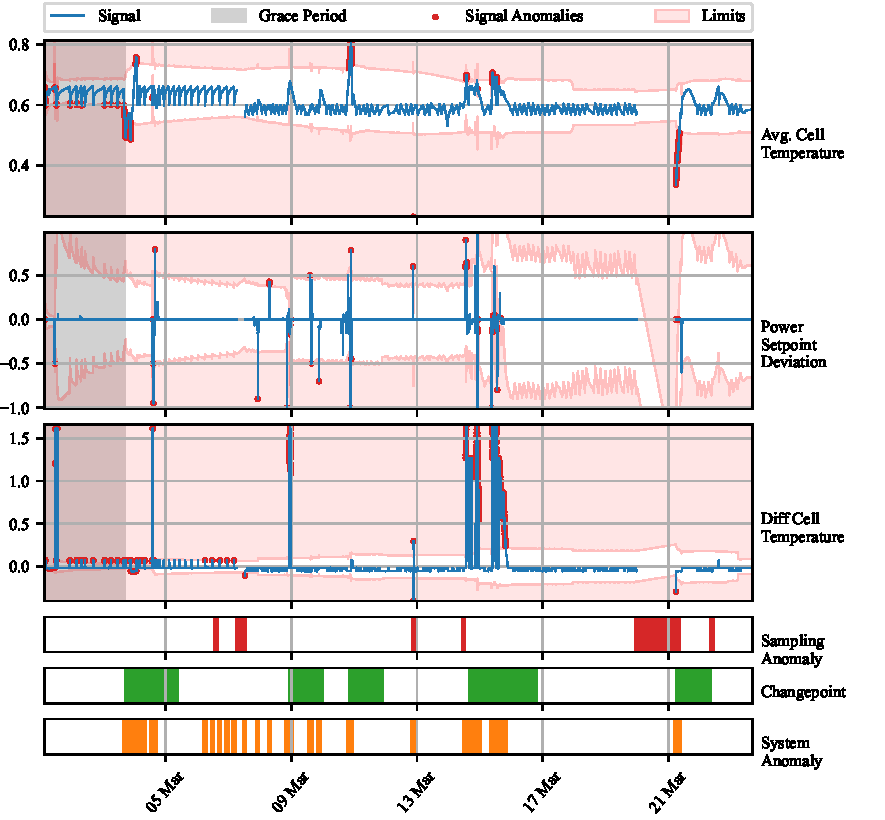
\includegraphics{figures/BESS_thresh.pdf}}
\caption{Time Series of BESS measurements (blue line) of process variables. The y-axis renders the values after the normalization of raw inputs. Root causes of anomalies are marked within specific signals as red dots. The light red area represents out-of-limits values for individual signals. Non-uniform sampling is marked as red bars. Green bars represent the times, at which changepoint was detected. All the signal anomalies are depicted as orange bars below the graph.}
\label{fig:bess}
\end{figure}

Fig. \ref{fig:bess} depicts the operation of the BESS over March 2022. Multiple events of anomalous behavior happened within this period, confirmed by the operators, that are observable through a sudden or significant shift in measurements in a given period. As the first step, the detection mechanism was initialized, following the provided guidelines for parameter selection in Subsection \ref{init}. The expiration period was set to $\ui{t}{e} = 7$ days, due to the weekly seasonality of human behavior impacting battery usage. The threshold was kept at default value $T = 0.99735$. A grace period, during which the model learns from both normal and anomalous data (though normal are expected), is shortened to 2.5 days to observe the effect of BESS calibration happening on 3\textsuperscript{rd} day from deployment.

The deployment and operation of the anomaly detection system were successful as shown by its adaptation of changepoint on 7\textsuperscript{th} March 2022 that appeared due to the relocation of the battery storage system outdoors. The model was adapted online based on Subsection \ref{train}. The sudden shift in environmental conditions, due to the transfer of the system to outside changed the dynamics of the system's temperature. However, new behavior was adopted by the top-level anomaly isolation system within five days, reducing potential false alerts afterward, by observably shifting the conditional mean to lower temperatures. Perhaps more interesting are the alerted changepoints.

Calibration of the BESS, usually observed as deviations of setpoint from real power demand and multiple peaks in temperature was captured as well.

The system identified 6 deviations in sampling, denoted by the red bars in Fig. \ref{fig:bess}. 4 anomalies with shorter duration represented packet loss. The prolonged anomaly was notified during the transfer of the battery pack. The longest dropout observed happened across 20\textsuperscript{th} March up to 21\textsuperscript{st}. Unexpectedly, the change point detection module triggered an alarm at the end of the loss, resulting in adaptation and a sharp shift in drawn limits for Power Setpoint Deviation. Red dots represent anomalies at the signal level given by equation \eqref{eq:anomaly_signal}. The dynamic signal limits are surpassed in one or multiple signals during the system's anomalies. The root cause isolation allows the pairing of anomalies with specific features. Conditional probability, against which the anomalies are evaluated allows consideration of signal relationships within individual limits.

\subsection{Kokam Battery Temperature Module(BESS)}\label{AA:Kokam}
A second case study is concerned with monitoring temperature profiles of individual modules of battery pack deployed at end user. During the operation, a hardware fault of the cooling fan happened. Our industrial partner was interested in finding out, whether such an event could be captured by an anomaly detection system. The data for 12 modules, each coming with 6 channels of measurement were retrieved in 30-second sampling and processed in a streamed manner. We found it informative to compute the deviation of the observed value from the average of all the above-mentioned measurements.

Our anomaly detection system was, once again, initialized with an expiration period of 7 days. The grace period was shortened to 1 day. The threshold value was shifted to a 4 sigma value of 99.977\% to minimize the number of alarms.

In Figure \ref{fig:kokam} we observe 5 days of deviations between the observed temperature measured by channels of module 9 and the average temperature of all modules. After the grace period, we observe multiple system alarms raised by various channels. Until the noon of 22\textsuperscript{nd} August, they seem to be spread out randomly between individual channels. During the late evening of 22\textsuperscript{nd}, anomalies were reported by both channels 4 and 5 for a prolonged period, followed by an anomalous rise in temperature measured by channel 6 early in the morning on 23\textsuperscript{rd} August. The fan fault was observed approximately at 5 pm on 23\textsuperscript{rd} August. Our anomaly detection system instantly raised an alarm, notifying us of anomalous behavior reported by channels 1 - 3. The prolonged duration of the alarm triggered the changepoint alarm approximately 2 hours later. This resulted in a slightly faster adaptation of the system to the new operation under increased temperature. Surprisingly, the temperature decreased during the next day, notifying us of the fan being in operation, to fail again 30 minutes later after the battery modules were cooled down to the previous setpoint. The anomaly detection system was triggered once again, although adaptation loosened the region of normal operation to allow itself to adapt. No significant anomalies in sampling were observed during the period.

\begin{figure}[htbp]
 \centerline{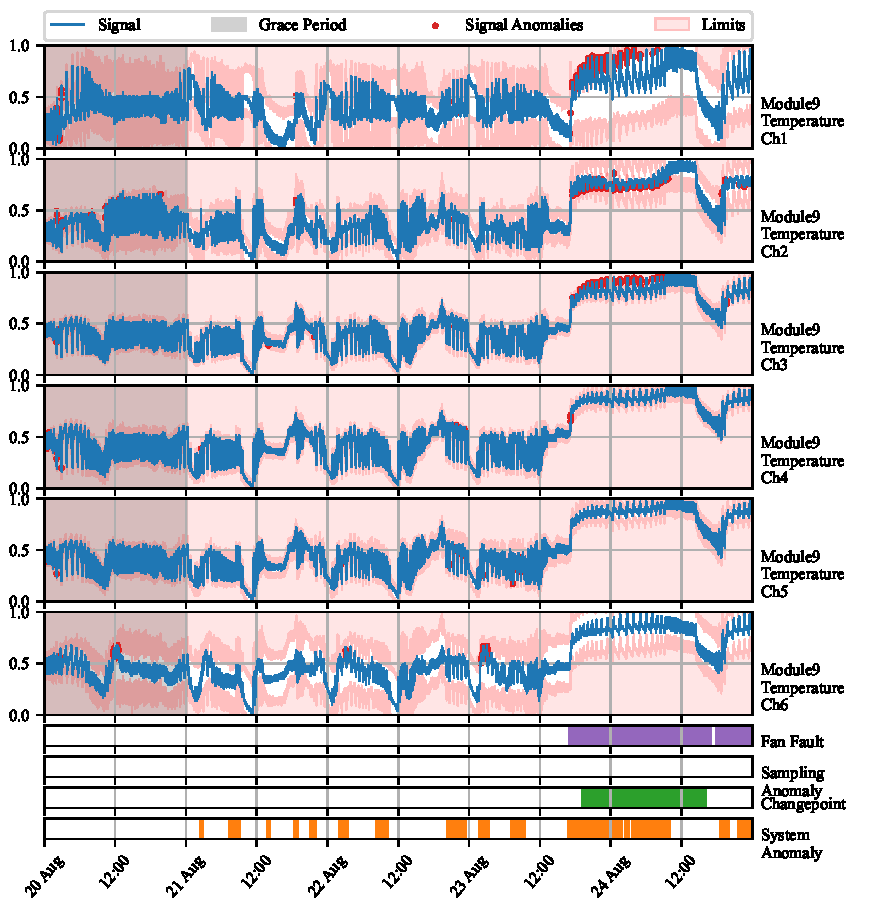
\includegraphics{figures/Kokam_thresh.pdf}}
 \caption{Time Series of BESS measurements (green line) of process variables. Non-uniform ticks on the x-axis mark days of interest (NOTE: some marks are hidden due to the readability). The y-axis renders the normalized process variables. System anomalies are marked as red dots. Non-uniform sampling is detected at blue vertical lines. Yellow vertical lines denote changepoint adaptation}
 \label{fig:kokam}
\end{figure}


\section{Conclusion}
In this paper, we demonstrate the capacity of adaptive conditional probability distribution to model the normal operation of dynamic systems employing streaming IoT data and isolate the root cause of anomalies. AID dynamically adapts to non-stationarity by updating multivariate Gaussian distribution parameters over time. Additionally, self-supervision enhances the model by protecting it from the effects of outliers and increasing the speed of adaptation in response to autonomously detected changes in operation.

Our statistical model isolates the root causes of anomalies as extreme deviations from the conditional means vector, considering spatial and temporal effects encoded in features, as demonstrated in our case studies. This approach establishes the system's operational state by analyzing the distribution of signal measurements, computing the distance from the mean of conditional probability, and setting dynamic operating limits based on multivariate distribution parameters. Additionally, the detector alerts for non-uniform sampling due to packet drops and sensor malfunctions. These adaptable limits can be seamlessly integrated into SCADA architecture, enhancing context awareness and enabling plug-and-play compatibility with existing infrastructure.

The ability to detect and identify anomalies in the system, isolate the root cause of anomaly to specific signal or feature, and identify signal losses is shown in two case studies on data from operated industrial-scale energy storages. These case studies highlight the model's ability to adapt, diagnose the root cause of anomalies, and leverage both physics-based models and spatially distributed sensors. Unlike many anomaly detection approaches, the proposed AID method does not require historical data or ground truth information about anomalies, alleviating the general limitations of detection methods employed in the energy industry.

The benchmark performed on industrial data indicates that our model provides comparable results to other self-learning adaptable anomaly detection methods. This is an important property of our model, as it also allows for root cause isolation.

AID represents a significant advancement in the safety and profitability of evolving systems that utilize well-established SCADA architecture and streaming IoT data. By providing dynamic operating limits, AID seamlessly integrates with existing alarm mechanisms commonly employed in SCADA systems. To the best of our knowledge, this study appears to be one of the initial attempts to introduce a self-supervised approach for adaptive anomaly detection and root cause isolation in SCADA-based systems utilizing IoT data streams.

Future work on this method will include improvements to the change point detection mechanism, reduction in latency for high-dimensional data, and minimizing the false positive rate, which is a challenge for general plug-and-play models. We will also explore the ability to operate with non-parametric models, in contrast to Gaussian distribution.


\bibliographystyle{IEEEtran}
\bibliography{main}

\end{document}
